% At least, use document class book
\documentclass[a4paper]{article}

\usepackage[T1]{fontenc}
\usepackage[latin1]{inputenc}
\usepackage{listings}
\usepackage{graphicx}
\usepackage{eso-pic}
\usepackage{pstricks}
\usepackage{listings}
\usepackage{graphicx}

\newcommand{\url}[1]{{\begin{ttfamily}#1\end{ttfamily}}}

\begin{document}

% Define the title of the thesis
\title{An Introduction into Dresden OCL2 for Eclipse}
% Specify the author of the thesis
\author{Claas Wilke and Ronny Brandt}
% Specify the date on which the thesis is handed in

\maketitle

This tutorial describes how the toolkit \textit{Dresden OCL2 for Eclipse} can be used. \textit{Dresden OCL2 for Eclipse} is the last version of the \textit{Dresden OCL Toolkit} and is based on the new infrastructure called the ``pivot model''. The pivot model was developed by Matthias Br�uer and is described in his ``Gro�er Beleg'' \cite{GBBraeuer}. Further information about the toolkit is available at the website of the \textit{Dresden OCL Toolkit} \cite{ToolkitHP}.

The tutorial starts with the installation of the needed \textit{Eclipse} plug-ins. Then it describes how to load a domain specific model and a model instance. Afterwords the importation and interpretation of OCL expressions will be explained.

The procedure described in this tutorial is realized and tested with \textit{Eclipse 3.4.1} \cite{Ecl}. The tutorial should also run with \textit{Eclipse 3.3.x}. Besides \textit{Eclipse} you also need to install some required plug-ins. Table \ref{tab:software} shows all required software to run \textit{Dresden OCL2 for Eclipse}.
  
\begin{table}
\begin{tabular}[h]{|p{5.2cm}|p{6cm}|}
    \hline
    \textbf{Software} & \textbf{Available at} \\
    \hline
    Eclipse 3.4.x & http://www.eclipse.org/ \\
    \hline
    Eclipse Modeling Framework (EMF) & http://www.eclipse.org/modeling/emf/ \\
    \hline
    Eclipse Model Development Tools (MDT) (only with the UML2.0 meta model) & http://www.eclipse.org/modeling/mdt/ \\
    \hline
    Supclipse plug-in (only to import the toolkit from the SVN) & http://subclipse.tigris.org/ \\
    \hline
    Eclipse Plugin Development Environment (only to run the toolkit using the source code distribution) & http://www.eclipse.org/pde/ \\
    \hline
\end{tabular}
\caption{Software needed to run \textit{Dresden OCL2 for Eclipse}.}
\label{tab:software}
\end{table}


	
\section{How to install Dresden OCL2 for Eclipse}
	
To use \textit{Dresden OCL2 for Eclipse} you need to install the toolkit as \textit{Eclipse} plug-ins, or to import them into your \textit{Eclipse workspace}. Both possibilities are explained in the following.
	
	
\subsection{Installing Dresden OCL2 for Eclipse as jar files}
	
To install \textit{Dresden OCL2 for Eclipse} as \textit{Eclipse} plug-in, you need to have the jar archives of the toolkit. The jar archives are available at \url{http://dresden-ocl.\linebreak[0]sourceforge.net/}. You need to copy the jar archives into the ``plugins'' directory of your \textit{Eclipse SDK} distribution. Then you can start the \textit{Eclipse SDK} and you can work with \textit{Dresden OCL2 for Eclipse}.
	
	
\subsection{Importing Dresden OCL2 for Eclipse into an Eclipse Workspace}

Alternatively you can import \textit{Dresden OCL2 for Eclipse} as plug-in projects into an \textit{Eclipse} workspace. There are two different options to do that.

On the one hand you can import the plug-ins from your file system, if you have already downloaded them (e.g. from \url{http://sourceforge.net/\linebreak[0]projects/\linebreak[0]dresden-ocl/} as a source code distribution). One the other hand you can import the plug-ins directly from the \textit{SVN} (\textit{Subversion}) of \textit{Dresden OCL2 for Eclipse}. Both possibilities are described below.

	
\subsubsection{Import the plug-ins from the local file system}
	
Let's say you have the plug-ins located in a directory \lstinline|XYZ| of your file system. To import them into your \textit{Eclipse} workspace you can use the \textit{Eclipse import wizard}. Open the wizard via the menu ``File > Import...'' and select  ``General > Existing Projects into Workspace'' (see figure \ref{pic:Import-EPiW}). In the following window you select the directory \lstinline|XYZ| as root. Then you select the plug-ins you want to import (if not selected automatically) and activate the check box ``Copy projects into workspace'' (see figure \ref{pic:ImportProjects}). After pressing the button ``Finish'' the plug-ins will be imported as projects into your workspace.
	
\begin{figure}
	\centering
	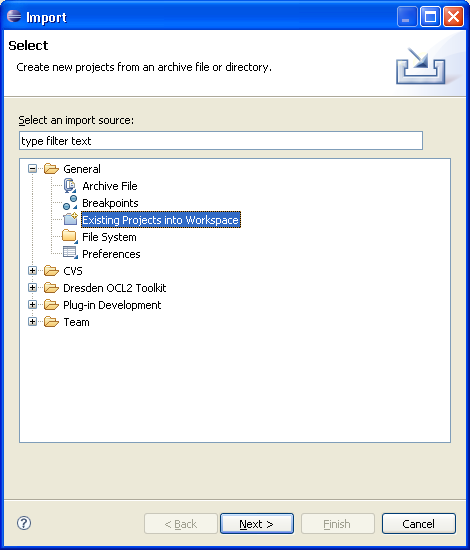
\includegraphics[width=0.8\linewidth]{figures/Import-EPiW}
	\caption{Plug-in import from local file system (1).}
	\label{pic:Import-EPiW}
\end{figure}
	
\begin{figure}[!htbp]
	\centering
	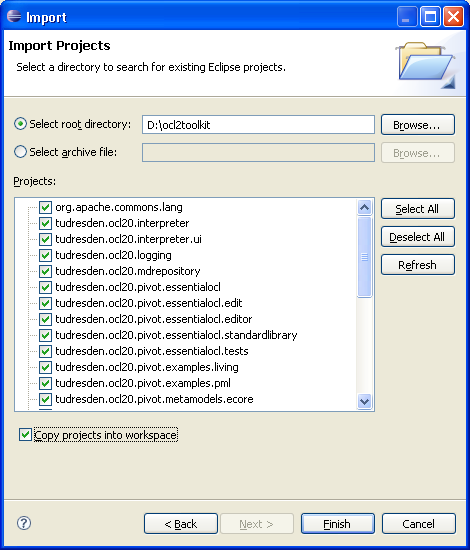
\includegraphics[width=0.8\linewidth]{figures/ImportProjects}
	\caption{Plug-in import from local file system (2) (not all required projects are shown in the picture).}
	\label{pic:ImportProjects}
\end{figure}
	
	
\subsubsection{Import the plug-in projects from SVN}
	
To import the plug-ins directly from the \textit{SVN} repository, you need to install an additionally \textit{Eclipse} plugin to connect with the \textit{SVN}. The needed plug-in is called \textit{Subclipse}. The installation of \textit{Subclipse} is explained on the \textit{Supclipse} website \cite{SVNInstall}.
	
\textbf{Attention: The \textit{Subclipse} plug-in does not work with some distributions of \textit{Eclipse 3.4}}. To access the \textit{SVN} Repository with \textit{Eclipse 3.4} use another \textit{SVN} plug-in for \textit{Eclipse} or use an external tool to access the \textit{SVN} repository.
	
After installing \textit{Subclipse}, a new \textit{Eclispe perspective} for access to \textit{SVN} should exist. The perspective can be opened via the menu ``Window > Open Perpective > Other... > SVN Repository Exploring''. In the view \textit{SVN Repository} you can add a new repository (see figure \ref{pic:SVN}) using the URL \url{https://dresden-ocl.\linebreak[0]svn.sourceforge.net/svnroot/dresden-ocl/}. After pressing the button\linebreak[0] ``Finish'' the SVN repository root should the visible in the \textit{repository view}.
	
To checkout the plug-ins, you now select them in the repository directory \url{trunk/ocl20forEclipse/eclipse} and use the ``Checkout...'' function in the context menu (see figure \ref{pic:Checkout}). The given settings could be used and after a click on the ''Finish'' button the plug-ins should be imported.
	
\begin{figure}[!htbp]
	\centering
	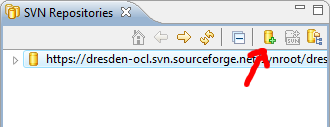
\includegraphics[width=0.5\linewidth]{figures/SVN}
	\caption{Adding an SVN repository.}
	\label{pic:SVN}
\end{figure}
	
\begin{figure}[!htbp]
	\centering
	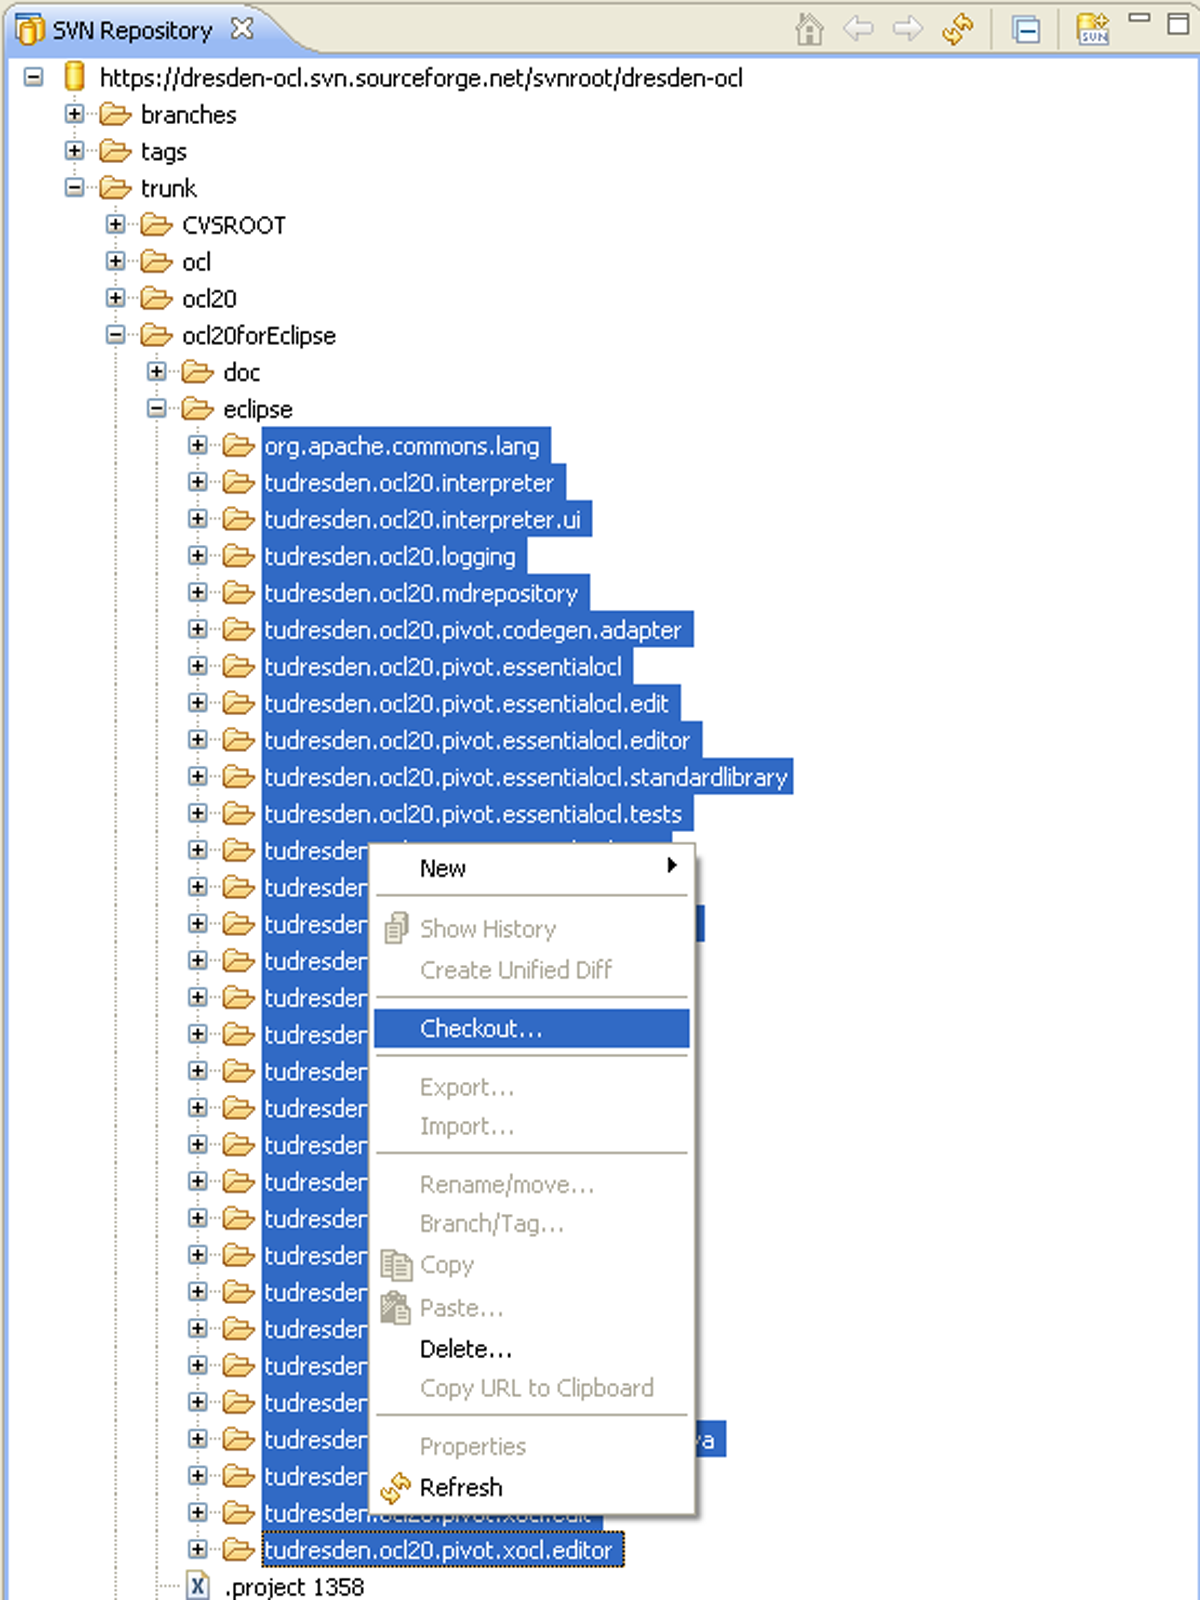
\includegraphics[width=1.0\linewidth]{figures/Checkout}
	\caption{Checkout of the Dresden OCL2 Toolkit plug-in projects (not all plug-ins are shown in the picture).}
	\label{pic:Checkout}
\end{figure}
	
	

\section{Building the OCL2 Parser}
	
If you decided to run \textit{Dresden OCL2 for Eclipse} as project plug-ins into your workspace, you need to build the \textit{OCL2 Parser} via an \textit{Ant} build script. If you installed the Toolkit using jar archives, you can skip this chapter of the tutorial.
  
To build the \textit{OCL2 Parser} select the file ``build.xml'' in the project ``tudresden.ocl20.pivot.ocl2parser'' and open the context menu via a right mouse click. Select the function ``Run As ... > Ant Build'' (see figure \ref{pic:Build}).

\begin{figure}[!htbp]
	\centering
	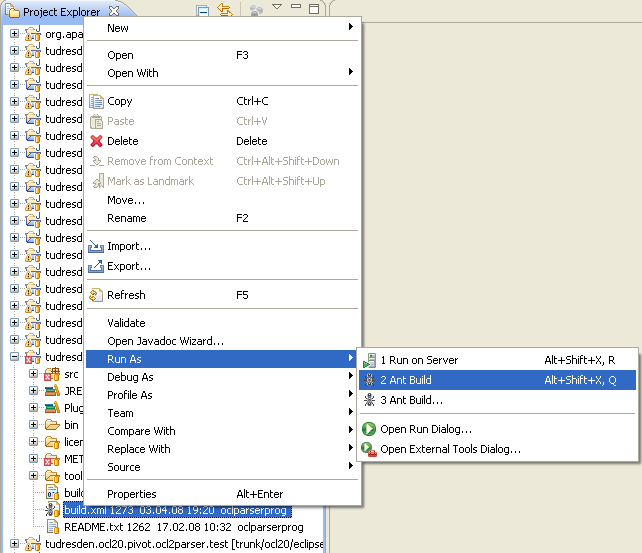
\includegraphics[width=1.0\linewidth]{figures/Build}
	\caption{Executing the OCL2 parser build script.}
	\label{pic:Build}
\end{figure}
	
If an error like ``Problem: failed to create task or type eclipse.refresh\-Local'' occurs, you need to change the configuration of the \textit{Ant} script. Open the function ``Properties'' in the context menu of the ``build.xml''. A new window should open. Select the topic ``Run/Debug settings'' and then the configuration for ``tudresden.ocl20.pivot.oclparser build.xml''. Click on the button ``Edit''. In the new window select in the sub menu ``JRE'' the check box ``Run in the same JRE as the workspace'' and click on the button ``OK'' (see figure \ref{pic:AntConfig}). Afterwords the \textit{Ant} script should be executable without errors.
	
\begin{figure}[!htbp]
	\centering
	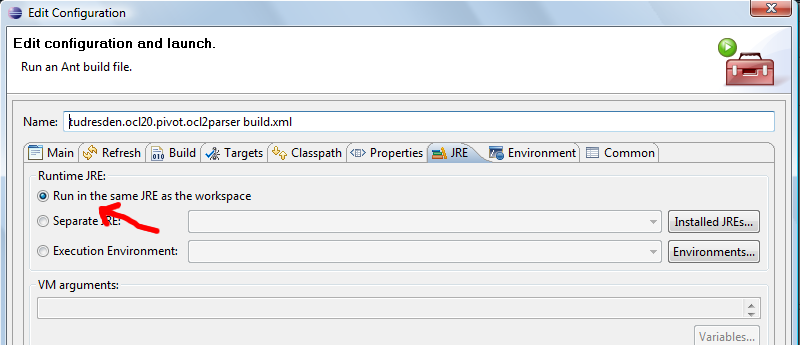
\includegraphics[width=1.0\linewidth]{figures/AntConfig}
	\caption{Settings of the JRE for the Ant build script.}
	\label{pic:AntConfig}
\end{figure}
	
After executing the build script successfully you need to update the projects in your workspace. Update the project \url{tudresden.ocl20.pivot.oclparser} via context menu (``Refresh'', see figure \ref{pic:Refresh}).

\begin{figure}[!htbp]
	\centering
	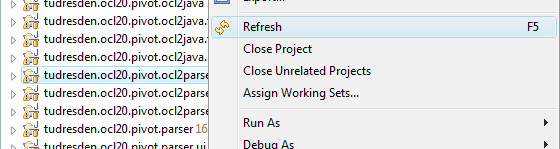
\includegraphics[width=0.5\linewidth]{figures/Refresh}
	\caption{Refreshing the project ``tudresden.ocl20.pivot.oclparser''.}
	\label{pic:Refresh}
\end{figure}
	
Additionally you need to recompile all depending projects. Select the function ``Project > Clean... > Clean all projects'' in the \textit{Eclipse} menu to clean all projects. All the projects should now contain no errors anymore and should be executable.


	
\section{Using Dresden OCL2 for Eclipse}

If you installed the \textit{Dresden OCL2 for Eclipse} using jar archives, you can execute the toolkit by starting your \textit{Eclipse SDK}. If you imported the Toolkit as plug-in projects into an \textit{Eclipse} workspace, you have to start a new \textit{Eclipse SDK} instance. You can start a new instance via the menu ``Run > Run As > Eclipse Application''. If the menu ``Eclipse Application'' is not available or disabled you need to select one of the plug-ins of the toolkit first.

This tutorial explains \textit{Dresden OCL2 for Eclipse} using the \textit{Simple example} which is located in the plug-in package \url{tudresden.ocl20.pivot.examples.\linebreak[0]simple}. Figure \ref{pic:Simple} shows the class diagram which is described by the \textit{Simple example}.

Table \ref{tab:examples} shows all examples which are provided with \textit{Dresden OCL2 for Eclipse} by now. The different examples use different meta models which is possible with the \textit{pivot-model} architecture of the toolkit. The \textit{Simple example} can be used with two different meta models. These are \textit{UML 1.5} (based on \textit{Netbeans MDR}) and \textit{UML 2.0} (based on \textit{Eclipse MDT UML2}).

\begin{figure}[!htbp]
	\centering
	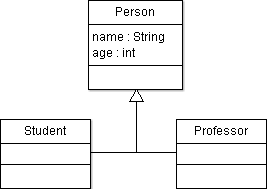
\includegraphics[width=0.5\linewidth]{figures/Simple}
	\caption{The class diagram described by the simple example model.}
	\label{pic:Simple}
\end{figure}

\begin{table}
\begin{tabular}[h]{|p{5.2cm}|p{6cm}|}
  \hline
  \textbf{Simple example} & \\
  Plug-in package & \url{tudresden.ocl20.pivot.examples.\linebreak[0]simple}\\
  Meta model & UML 1.5 or UML 2.0\\
  Model & \url{model/simple.xmi} (with UML 1.5) \newline \url{model/simple.uml} (with UML 2.0)\\
  OCL expressions & \url{constraints/invariants.ocl}\\
  Model instance & \url{src/tudresden.ocl20.pivot.\linebreak[0]examples.simple/\linebreak[0]ModelProviderClass.java}\\
  \hline
  \hline
  \textbf{Living example} & \\
  Plug-in package & \url{tudresden.ocl20.pivot.examples.\linebreak[0]living}\\
  Meta model & UML 1.5\\
  Model & \url{model/UmlExample.xmi}\\
  OCL expressions & \url{expressions/living.ocl}\\
  Model instance & \url{src/tudresden.ocl20.pivot.\linebreak[0]examples.living/\linebreak[0]ModelProviderClass.java}\\
  \hline
  \hline
  \textbf{PML example} & \\
  Plug-in package & \url{tudresden.ocl20.pivot.examples.\linebreak[0]pml}\\
  Meta model & Ecore\\
  Model & \url{model/pml.ecore}\\
  OCL expressions & \url{expressions/testpml.ocl}\\
  Model instance & \url{model instance/Testmodell.pml}\\
  \hline
\end{tabular}
\caption{Examples provided with \textit{Dresden OCL2 for Eclipse}.}
\label{tab:examples}
\end{table}
	
	
\subsection{Loading a domain specific model}
	
After starting \textit{Eclipse} you have to load a model into the toolkit. 

If the plug-ins of \textit{Dresden OCL2 for Eclipse} were installed as jar archives, the \textit{Simple example} plug-in has to be imported into the \textit{Workspace} first. Create a new Java project into your \textit{Workspace} and select the \textit{import wizard} ``General -> Archive File''; in the following window select the ``plugins'' directory into your \textit{Eclipse} root folder, select the archive \url{tudresden.ocl20.pivot.examples.\linebreak[0]simple\_1.0.0.jar} and click the ``Finish'' button.

Now you can load a model by using the \textit{import wizard} (File~>~Import...). Select the wizard ``Dresden OCL2 Toolkit > Domain-Specific~Model''. In a new opened window you have to select a model file and a meta model for the model (see figure \ref{pic:LoadModel}). Click the button ``Browse Workspace...'' and select the file \url{model/simple.uml} inside the \textit{Simple example project}. Then select the meta model \textit{UML2} and press the button ``Finish''.

\begin{figure}[!htbp]
	\centering
	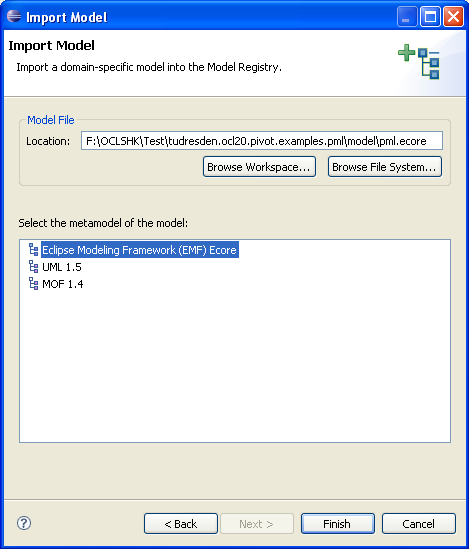
\includegraphics[width=0.8\linewidth]{figures/LoadModel}
	\caption{Loading a domain specific model.}
	\label{pic:LoadModel}
\end{figure}
	
Figure \ref{pic:MoBrOE} shows the loaded \textit{simple} model, which uses \textit{Ecore} as its meta model. Via the menu button (the little triangle in the right top corner) you can switch between different models in the model browser (see figure \ref{pic:SwitchModel}).
	
\begin{figure}[!htbp]
	\centering
	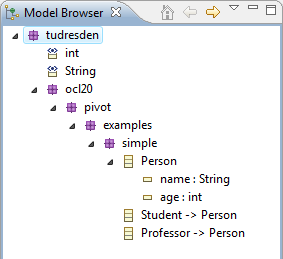
\includegraphics[width=0.5\linewidth]{figures/MoBrOE}
	\caption{The loaded simple example model in the model browser.}
	\label{pic:MoBrOE}
\end{figure}

\begin{figure}[!htbp]
	\centering
	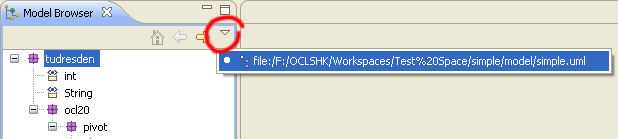
\includegraphics[width=1.0\linewidth]{figures/SwitchModel}
	\caption{You can switch between different models using the little triangle.}
	\label{pic:SwitchModel}
\end{figure}

	
\subsection{Loading a model instance}
	
After loading the model, you can load a \textit{model instance} using another \textit{import wizard}. Use the wizard ``Dresden OCL2 Toolkit > Model Instance''. You have to select a model instance (in this tutorial we used the file \url{bin/tudresden/ocl20/\linebreak[0]pivot/examples/ModelProviderClass.class} of the \textit{simple example} and the domain specific model loaded before (see figure \ref{pic:LoadInstance}).

\begin{figure}[!htbp]
	\centering
	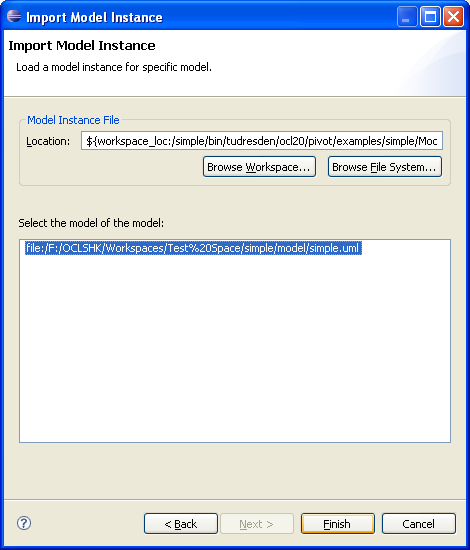
\includegraphics[width=0.8\linewidth]{figures/LoadInstance}
	\caption{Loading a simple model instance.}
	\label{pic:LoadInstance}
\end{figure}
	
Figure \ref{pic:MoInBr} shows the loaded model instance of the \textit{simple example} model. Like in the model browser you can switch between different model instances. Note that the model instance browser only shows the model instances of the model actually selected in the model browser. By switching the domain specific model, you also switch the pool of model instances available in the model instance browser.

\begin{figure}[!htbp]
	\centering
	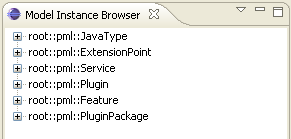
\includegraphics[width=0.5\linewidth]{figures/MoInBr}
	\caption{A simple model instance in the Model Instance Browser.}
	\label{pic:MoInBr}
\end{figure}

	
\subsection{Loading OCL expressions}
\indent
	
Before you can interprete OCL constraints you have to load them like the domain specific model and the model instance before. Use the import wizard ``Dresden OCL2 Toolkit > OCL Expressions'' and select an OCL file (in this tutorial we used the OCL file \url{constraints/invariants.ocl} of the \textit{simple example}, see figure \ref{pic:LoadExpressions}). The constraints of the file \url{constraints/invariants.ocl} are shown in listing \ref{list:invariants}.

\begin{figure}[!htbp]
	\centering
	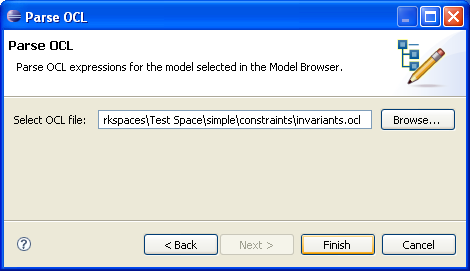
\includegraphics[width=0.8\linewidth]{figures/LoadExpressions}
	\caption{The import of OCL expressions.}
	\label{pic:LoadExpressions}
\end{figure}
	
\lstset{
  caption={The invariants of the simple examples.},
  frame=single,
  basicstyle=\small, 
  basicstyle=\scriptsize,
  keywords={package, context, inv, not},
  keywordstyle={\bfseries}
}
\begin{lstlisting}[label=list:invariants, breaklines=true]
package tudresden::ocl20::pivot::examples::simple

-- The age of Person can't be negative.
context Person
inv: age >= 0

-- Students should be 16 or older.
context Student
inv: age > 16

-- Proffesors should be at least 30.
context Professor
inv: not (age < 30)

endpackage
\end{lstlisting}

	
The expressions of the selected OCL file will be loaded into the actually selected model instance. Figure \ref{pic:MoBrME} shows the  ``Model Browser'' containing the model and the parsed expressions.
	
\begin{figure}[!htbp]
	\centering
	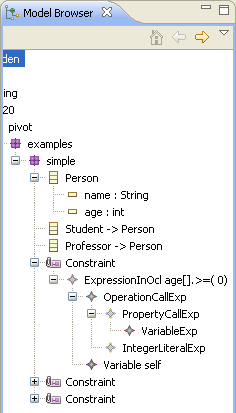
\includegraphics[width=0.5\linewidth]{figures/MoBrME}
	\caption{Parsed expressions and the model in the Model Browser.}
	\label{pic:MoBrME}
\end{figure}
	
	
\subsection{Interpretation of constraints}
\indent
	
The interpretation of constraints is possible via the \textit{Interpreter View}. Eventually you have to open the \textit{View} via the menu option ``Window -> Show View -> Other...'' and select ``TU Dresden OCL2 Toolkit -> Interpreter''.
	
The \textit{Interpeter View} provides a context menu containing all needed functionality. The context menu is shown in figure \ref{pic:IntViewMen} (You can open the context menu via the little triangle in the right top corner of the \textit{Interpreter View}).
	
\begin{figure}[!htbp]
	\centering
	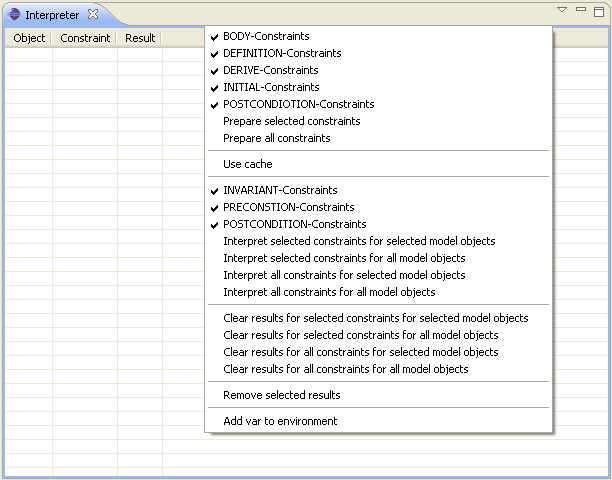
\includegraphics[width=1\linewidth]{figures/IntViewMen}
	\caption{The context menu of the \textit{Interpreter View}.}
	\label{pic:IntViewMen}
\end{figure}
	
For the interpretation of constraints you can use the functions ``Interpret~...'' in the context menu. First you can select constraints you want to interpret in the \textit{Model Browser} and the model objects for which the constraints should be interpreted in the \textit{Model Instance Browser}. The \textit{Model Instance Browser} shows only the model objects, for which you can interpret the constraints selected before.
	
In the \textit{interpreter menu} you can select the types you want to interpret (invariants, pre and post conditions). After interpretation the table in the \textit{Interpreter View} shows all results. These are filtered by the selection of constraints and model objects. Figure \ref{pic:IntView} shows a table with some results. If the column ``Result'' does not contain enough space for a result, you can open a result via a double mouse click in a new window.
	
\begin{figure}[!htbp]
	\centering
	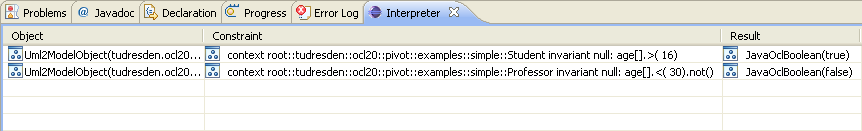
\includegraphics[width=1\linewidth]{figures/IntView}
	\caption{Some results in the \textit{Interpreter View}.}
	\label{pic:IntView}
\end{figure}

	

\section{Conclusion}
  
This tutorial described how to use \textit{Dresden OCL2 for Eclipse}. It explained how to install or import and start the Toolkit's plug-ins. Afterwords the usage of the interpreter of \textit{Dresden OCL2 for Eclipse} was shown.
  	
As mentioned before, more information about \textit{Dresden OCL2 for Eclipse} is available at the website of \textit{Dresden OCL Toolkit} \cite{ToolkitHP}.



\newpage
\bibliographystyle{alphadin}
\bibliography{tutorial_eng}

\end{document}
